\section{Algoritmo di Prim}\label{prim}

\begin{lstlisting}[mathescape=true]
PRIM (G, s)
	X = {s} //set of vertexes included in the MST
	A = $\emptyset$ //set of edges included in the MST
	while there is an edge (u, v) with u $\in$ X and v $\notin$ X do
		(u$\ast$, v$\ast$) = a minimum cost such edge //light edge
		add vertex v$\ast$ to X
		add edge (u$\ast$, v$\ast$) to A
	return A	

\end{lstlisting}

L'algoritmo di Prim costruisce un MST a partire da un vertice di iniziale $s$, aggiungendoci un lato alla volta:

\begin{figure}[H]
	\centering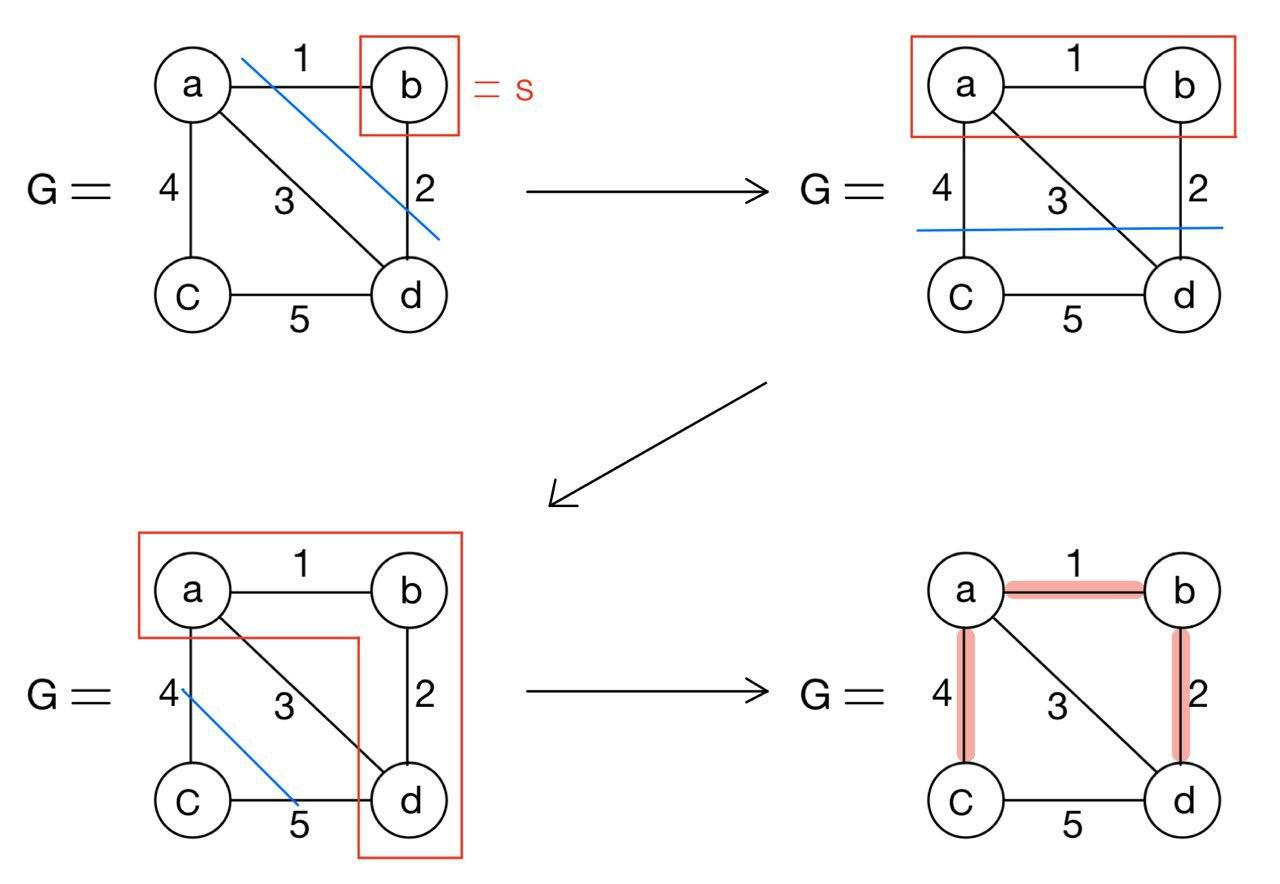
\includegraphics[width=15cm]{Img/prim.jpg}
\end{figure}

Ad ogni iterazione, si considerano i lati attraversati dal taglio (raffigurato in blu) che separa $X$ dal resto del grafo. 
Successivamente, di questi viene scelto il lato $(u, v)$ di peso minimo. 
Infine, il lato selezionato viene aggiunto all'insieme $A$ e il vertice $v$ viene aggiunto all'insieme $X$.

\subsection{Strutture dati}
	
	\subsubsection{MinHeap}
		La struttura dati utilizzata per l'implementazione dell'algoritmo è la struttura \textit{min-heap}. 
		Un \emph{MinHeap} è un oggetto composto da un array che può essere considerato come un albero binario quasi completo. 
		Ogni nodo dell'albero corrisponde a un elemento dell'array. 
		Tutti i livelli sono completamente riempiti, tranne eventualmente l'ultimo che può essere riempito da sinistra fino ad un certo punto.\\
		Un array \texttt{A} che rappresenta un heap è un oggetto \emph{ArrayHeap}, il quale estende la classe \emph{List} e presenta attributi:
		\begin{itemize}
			\item \texttt{A.length}: numero degli elementi dell'array;
			\item \texttt{A.heap-size}: numero degli elementi dell'heap che sono registrati nell'array.
		\end{itemize}
		Cioè, anche se ci possono essere dei numeri memorizzati in tutto l'array \texttt{A[1 ... A.length]}, soltanto i numeri in \texttt{[1 ... A.heap-size]}, dove $0 \leq$ \texttt{A.heap-size} $\leq$ \texttt{A.length}, sono elementi validi dell'heap.\\
		A partire dall'indice $i$ di un nodo è possibile accedere all'indice del padre, del figlio sinistro e del figlio destro nel seguente modo:
		\begin{itemize}
			\item \texttt{parent(i)}: $\lfloor i/2 \rfloor$ 
			\item \texttt{left(i)}: $2 \ast i$
			\item \texttt{right(i)}: $2 \ast i + 1$
		\end{itemize}
		Un \textit{min-heap} presenta la cosiddetta proprietà del \textit{min-heap}, secondo la quale, per ogni nodo diverso dalla radice, si ha che \texttt{A[parent(i)] $\leq$ A[i]}. Di conseguenza il più piccolo elemento in un min-heap è nella radice.
		Le altre informazioni relative all'oggetto \emph{MinHeap} sono le seguenti:
		\begin{itemize}
				\item \texttt{\textbf{minHeapify(i)}}: metodo che permette di mantenere la proprietà del min-heap a partire dall'indice \texttt{i};
				\item \texttt{\textbf{bubbleUp(i)}}: metodo che permette di mantenere la proprietà del min-heap, riposizionando l'elemento di indice \texttt{i} dell'array-heap nella posizione corretta, risalendo di padre in padre;
				\item \texttt{\textbf{extractMin()}}: metodo che estrae il minimo dall'array-heap, cioè la radice dell'albero, e ristabilisce la proprietà del min-heap tramite la chiamata a \texttt{minHeapify(i)}.
		\end{itemize}
		
	\subsubsection{Node}
	L'oggetto \textit{Node} rappresenta un vertice del grafo. 
	Esso comprende i seguenti campi dati:
	\begin{itemize}
		\item \texttt{\textbf{tag}}: intero che identifica un vertice;
		\item \texttt{\textbf{key}}: chiave del vertice, il suo valore di default è \texttt{None};
		\item \texttt{\textbf{parent}}: padre del vertice, il suo valore di default è \texttt{None};
		\item \texttt{\textbf{isPresent}}: variabile booleana che memorizza la presenza di un nodo nell'array che rappresenta l'heap. Il suo valore di default è \texttt{True};
		\item \texttt{\textbf{index}}: indice dell'array del min-heap associato al vertice; 
		\item \texttt{\textbf{adjacencyList}}: lista di adiacenza del vertice, il suo valore di default è la lista vuota.
	\end{itemize}
	
	\subsubsection{Graph}
		L'oggetto \textit{Graph} permette di gestire la creazione e la costruzione di un grafo secondo le caratteristiche specificate nel file \texttt{.txt} dato in input. 
		Il suo unico campo dati è \texttt{nodes}, un dizionario di oggetti di tipo \texttt{Node}. 
		Il tipo dizionario utilizzato è \texttt{defaultDict} di Python. 
		La scelta di utilizzare questo tipo di dizionario è dovuta al fatto che l'oggetto viene inizializzato con una funzione che fornisce un valore di default nel caso si utilizzi una chiave non esistente. 
		In questo modo non vengono sollevate eccezioni del tipo \textit{``KeyError''}.\\
		Le altre informazioni relative all'oggetto \emph{Graph} sono le seguenti:
		\begin{itemize}
			\item \texttt{\textbf{createNodes(n)}}: metodo che instanzia \texttt{n} vertici nel dizionario \texttt{nodes};
			\item \texttt{\textbf{addNode(u, v, cost)}}: metodo che aggiorna le liste di adiacenza dei nodi \texttt{u} e \texttt{v}, inserendo inoltre, in entrambe, il peso dell'arco che li collega;
			\item \texttt{\textbf{buildGraph(n)}}: metodo principale per la costruzione del grafo. Esso prima chiama il metodo \texttt{createNodes(n)}  e, successivamente, il metodo \texttt{addNode(u, v, cost)} per ogni vertice di input.
		\end{itemize}

\subsection{Implementazione}

	La soluzione del problema è stata implementata nel seguente modo:
	
	\begin{itemize}
		\item Viene inizializzato il grafo $G$ attraverso il metodo \texttt{buildGraph()}, al quale viene passato il grafo di input come parametro. 
		La funzione esegue due passaggi in sequenza:
		\begin{enumerate}
			\item Tramite l'apposito costruttore, vengono inizializzati nel dizionario del grafo un numero di vertici uguale a quanto indicato nella prima riga dell'input. La chiave per accedere ad un vertice è il suo \texttt{tag};
			\item Per ogni tripla ($vertice_1\_arco_i$, $vertice_2\_arco_i$, $peso\_arco_i$) dell'input, vengono aggiornate le liste di adiacenza di entrambi i vertici poiché il grafo è indiretto:
			
			\texttt{nodes[tag\_vertice1].adjacencyList.append([nodes[tag\_vertice2], peso])}
			\texttt{nodes[tag\_vertice2].adjacencyList.append([nodes[tag\_vertice1], peso])}
			
			Ogni lista di adiacenza, quindi, contiene un numero di sottoliste di due elementi pari al numero di vertici adiacenti. 
			I due elementi sono il vertice adiacente e il peso dell'arco che connette i due vertici. 
			In questo modo si riesce ad accedere sia alle informazioni del vertice adiacente sia al peso in maniera immediata.\\
			L'inizializzazione al punto $1$ tutti i possibili vertici del grafo assicura che il vertice che viene aggiunto alla lista di adiacenza di un altro vertice sia un oggetto definito. 
			Inoltre ogni vertice presente in una lista di adiacenza è un riferimento all'oggetto vero e proprio. 
			In questo modo non vengono effettuate copie inutili;
		\end{enumerate}
	
	\item Una volta creato il grafo, questo viene fornito come input all'algoritmo \texttt{MSTPrim} insieme al nodo di partenza. 
	L'algoritmo esegue i seguenti passi:
	\begin{enumerate}
		\item Assegna al campo \texttt{key} di ogni vertice il valore $\infty$ \texttt{(math.inf)};
		\item Assegna al campo \texttt{key} del nodo di partenza il valore $0$;
		\item Viene inizializzata la struttura min-heap a partire dai nodi del grafo. 
		L'inizializzazione tiene conto del nodo di partenza. 
		Infatti, seguendo la struttura del file di input, la lista di vertici che viene fornita come input alla struttura dati è una lista ordinata a partire dal vertice con \texttt{tag = 1}. 
		Di conseguenza possono verificarsi due casi:
		\begin{itemize}
			\item Se il vertice di partenza è il vertice con \texttt{tag = 1} quest'ultimo sarà il nodo radice dell'albero min-heap, in quanto il suo campo \texttt{key}, utilizzato per confrontare i nodi, sarà il più piccolo. 
			In questo caso l'array-heap sarà costruito utilizzando la lista di input;
			\item Se il vertice di partenza ha \texttt{tag != 1} l'array-heap viene costruito in modo analogo a prima. 
			Dopodiché il nodo di partenza viene posto in testa all'array-heap e tutti i campi \texttt{index} di tutti vertici vengono aggiornati.
			\begin{figure}[H]
				\hspace{-1cm}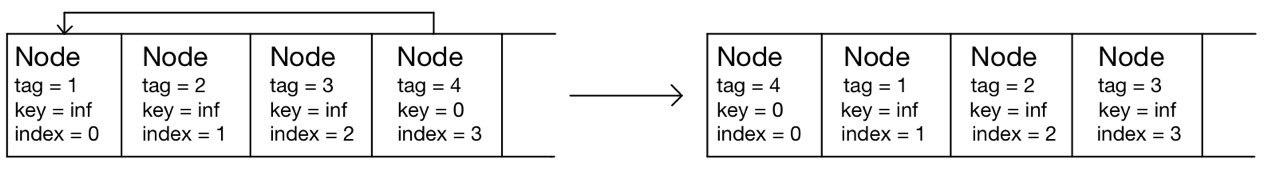
\includegraphics[width=18.5cm]{Img/arrayheap.jpg}
			\end{figure}
		\end{itemize}
		Posizionare il nodo di partenza in testa all'array-heap assicura che la proprietà del min-heap venga rispettata. 
		Il compromesso è l'aggiornamento di tutti i campi \texttt{index}, eseguibile in tempo lineare nel numero di vertici;
		\item A questo punto comincia la fase iterativa dell'algoritmo:
		\begin{enumerate}
			\item Viene estratto il minimo dalla struttura min-heap tramite la procedura \texttt{extractMin()}. 
			Per fare ciò essa estrae la radice dell'albero, effettua gli aggiornamenti necessari per mantenere la proprietà del min-heap attraverso il metodo \texttt{minHeapify()}, assegna al campo \texttt{isPresent} il valore \texttt{false} poiché il vertice non farà più parte dell'array-heap ed infine ritorna la radice;
			\item Per ogni vertice \texttt{v} nella lista di adiacenza del vertice appena estratto si controlla che i) appartenga all'array-heap e ii) che il peso dell'arco tra i due sia minore del valore attuale del campo \texttt{key} del vertice estratto. 
			In caso positivo, si procede all'aggiornamento dei campi \texttt{parent} e \texttt{key} di \texttt{v};
			\item Viene invocato il metodo \texttt{bubbleUp()} per mantenere la proprietà del min-heap. 
			Esso colloca nella posizione esatta dell'albero il vertice \texttt{v} in quanto il suo campo \texttt{key} è stato precedentemente aggiornato.
		\end{enumerate} 
	\end{enumerate}
\end{itemize}

\subsection{Complessità}
	La complessità dell'algoritmo è $O(m\log(n))$, dove $m$ indica il numero totale di archi e $n$ il numero totale di vertici:
	\begin{itemize}
		\item L'inizializzazione della struttura min-heap, nel caso peggiore, richiede un tempo di esecuzione $O(n)$;
		\item L'operazione \texttt{extractMin()} ha un tempo di esecuzione di $O(\log(n))$ e viene ripetuta $n$ volte all'interno del ciclo \texttt{while}. Il costo totale quindi è $O(n\log(n))$;
		\item Il ciclo \texttt{for} viene eseguito $O(m)$ volte, in quanto la somma delle lunghezze delle liste di adiacenza è $2|m|$. All'interno del ciclo \texttt{for}, il test che verifica l'appartenenza di un vertice adiacente alla struttura min-heap è eseguito in tempo costante $O(1)$. 
		Infine, l'operazione \texttt{bubbleUp()} per il ripristino della proprietà del min-heap è eseguita in tempo $O(\log(n))$. 
		Il costo totale quindi è $O(m\log(n))$;
	\end{itemize}
	Sommando questi dati il tempo totale dell'algoritmo è $O(n\log(n) + m\log(n))) = O(m\log(n))$.
	
\pagebreak